The database is a persistence provider providing long term, organized storage
of the data which will be generated through the application. Various types of
database exist, which are mainly categorized based on the approach with which
the provider in questions represents and stores the data internally. Some of 
the types of databases which where considered for this project include
\begin{itemize}
	\item Relational Databases e.g. MySQL, PostgreSQL
	\item Document-oriented Databases e.g. MongoDB, Couchbase
	\item Graph-based Databases Neo4j, OrientDB
\end{itemize}

In choosing a persistence provider, it is important to consider the data as
well as the relationship between the data to ensure the correct type of 
provider is selected.

The data to be generated by the benchmarking service will have a very flat
relationship structure between data elememtns. This flat structure naturally
makes the data well suited for a document-based persistence provider.

\subsection{Architecture Requirements}
\subsubsection{Access and Integration Requirements}
\subsubsection{Quality Requirements}
\paragraph{Scalability}
The database selected must allow for horizontal scaling of the infrastructure,
which means that the database should be able to scale across different hosts to
form a combined and intelligant cluster. Optional support of distribution the
database across providers will be benefical for future expansion.

\paragraph{Performance}
As the database will receive a higher ratio of reading to writing operations
per sec, this must be kept in mind when selecting the required database. The
database should also be able to deliver on strict Service Level Agreements
(SLA), especially on availability.

\paragraph{Reliability}
As the database will be used to build a repository of knowledge, in the form of
historical benchmark results and test data sets, it is of the utmost importance
that the selected database store is able to preserve data reliably even in the
event of a possible disaster. The one again highlights the need for a database
store which is able to function across data centers.

\paragraph{Integrability}
The chosen database should be supporte by the chosen perisistence API realization
in such a way, that from the business logic, there are no database specific
code. The chosen persistence API was chosen for this exact reason as to support
the swapping out of the underlying database store without the need to change any
higher level code. As not all databases are supported by the persistence API,
this places an inherit technological constraint on the database stores which can
be utilized in the project.

\paragraph{Deployability}
This requirement places no further restrictions on the requirements as set out
in section \ref{sec:systemDeployability}.

\subsubsection{Architectural Responsibilities}
The architectural responsibilities of the database are shown in 
Figure \ref{fig:databaseResponsibilities}
\begin{figure}[H]
	\begin{center}
	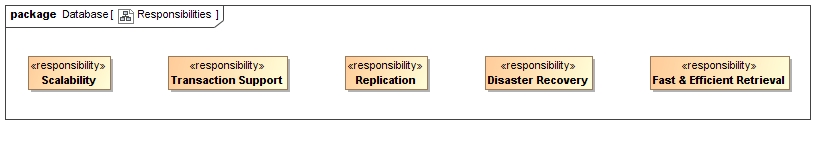
\includegraphics[scale=0.5]{../Diagrams and Charts/Database/Responsibilities.jpg}
	\caption{The architectural responsibilities of the Database}
	\label{fig:databaseResponsibilities}
	\end{center}
\end{figure}

\subsubsection{Architecture Constraints}
\subsection{Architecture Design}
\subsubsection{Tactics}
Tactics which should be used by the database to address the quality requirements:
\begin{itemize}
	\item \textit{Scaling out resources} to allow for flexiable and cheap
		improvement in performance and scalability.
	\item \textit{Efficient Persistence} to allow for the quick and efficient
		retrieval of data from the provider aiding in performance
		improvement.
	\item \textit{Efficient Storage Usage} to minimize the required
	infrastructure needed by the service.
	\item \textit{Spread Load} in order to fulfill the required scalability
		and performance requirements as set out above.
	\item \textit{Removing single points of failure} to ensure data is
		protected against disasters as the client will be building a
		knowledge repository.
\end{itemize}

\subsubsection{Architectural Components}
The architectural components of the database are shown in 
Figure \ref{fig:databaseResponsibilityAllocation}
\begin{figure}[H]
	\begin{center}
	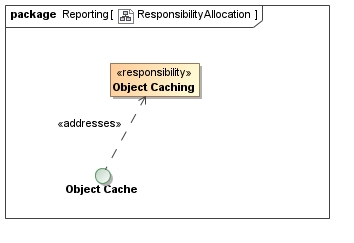
\includegraphics[scale=0.5]{../Diagrams and Charts/D/ResponsibilityAllocation.jpg}
	\caption{The architectural responsibilities of the Database}
	\label{fig:databaseResponsibilityAllocation}
	\end{center}
\end{figure}

\subsubsection{Frameworks and Technologies}
\paragraph{Concrete Realization of Architectural Components}
\paragraph{Tactics}
\paragraph{Tools}
\paragraph{Concepts and Constraints for Application Components}